\section{Background}

This section introduces the core concepts of RabbitMQ and notable protocols that are relevant to the benchmark experiments presented in this paper. We first describe the AMQP messaging model and how RabbitMQ implements it, then explain how Quorum Queues use the Raft consensus algorithm to provide data safety through replication.

\subsection{RabbitMQ and AMQP}
RabbitMQ is an open-source message broker that implements the Advanced Message Queuing Protocol (AMQP)~\cite{amqp_spec}, \cite{rmq_amqp_docs}. In AMQP, publishers send messages to an \textit{exchange}, which routes them to one or more \textit{queues} based on configurable \textit{bindings} and routing keys. Consumers then read messages from queues. This indirection decouples producers from consumers where neither side needs to be aware of the other and messages can be buffered in queues when consumers are temporarily unavailable~\cite{Magnoni_2015}.

A RabbitMQ cluster consists of multiple nodes that share metadata about exchanges, queues and bindings. Clients can connect to any node in the cluster. When a client publishes to or consumes from a queue whose data resides on a different node, the receiving node proxies the operation to the node that owns the queue~\cite{rmq_clustering_docs}. This proxy path adds an extra network hop compared to connecting directly to the queue leader node.

\subsection{Quorum Queues and Raft}
Classic Mirrored Queues were RabbitMQ's former queue type for queue replication across cluster nodes. However, they had significant shortcomings regarding data consistency: the replication algorithm could produce message loss and administrators were forced to choose between availability and data safety during network partitions~\cite{rmq_ha_upgrade_blog}. Quorum Queues were introduced as a replacement and are now the recommended queue type for workloads that require data safety and high availability.

Under the Raft consensus algorithm~\cite{raft_paper}, each quorum queue is implemented as a replicated state machine with one replica on each cluster node, where one serves as the \textit{leader} and the rest as \textit{followers}. The leader handles all reads and writes for the queue. When a publisher sends a message, the leader appends it to its local write-ahead log (WAL) and replicates the entry to all followers. The message is only considered committed once a \textit{majority} of members (the quorum) have persisted the entry. The leader only acknowledges the message back to the publisher once the commit is complete.

The quorum for a cluster of size $n$ is $\lfloor n/2 \rfloor + 1$. This means a three-node cluster tolerates one node failure (quorum of two), a five-node cluster tolerates two (quorum of three) and so on. While adding nodes increases fault tolerance, it also increases the number of acknowledgements required before a message is committed. Each additional member that must persist a log entry adds further disk I/O and network round trips to the commit path, which reduces overall queue throughput as the cluster grows~\cite{rmq_quorum_docs}. The effect of this replication overhead on throughput and end-to-end latency as the cluster grows is the central question of this work. Figure~\ref{fig:raft_replication} illustrates the replication process for a six-node quorum queue.

\begin{figure}[!ht]
\centering
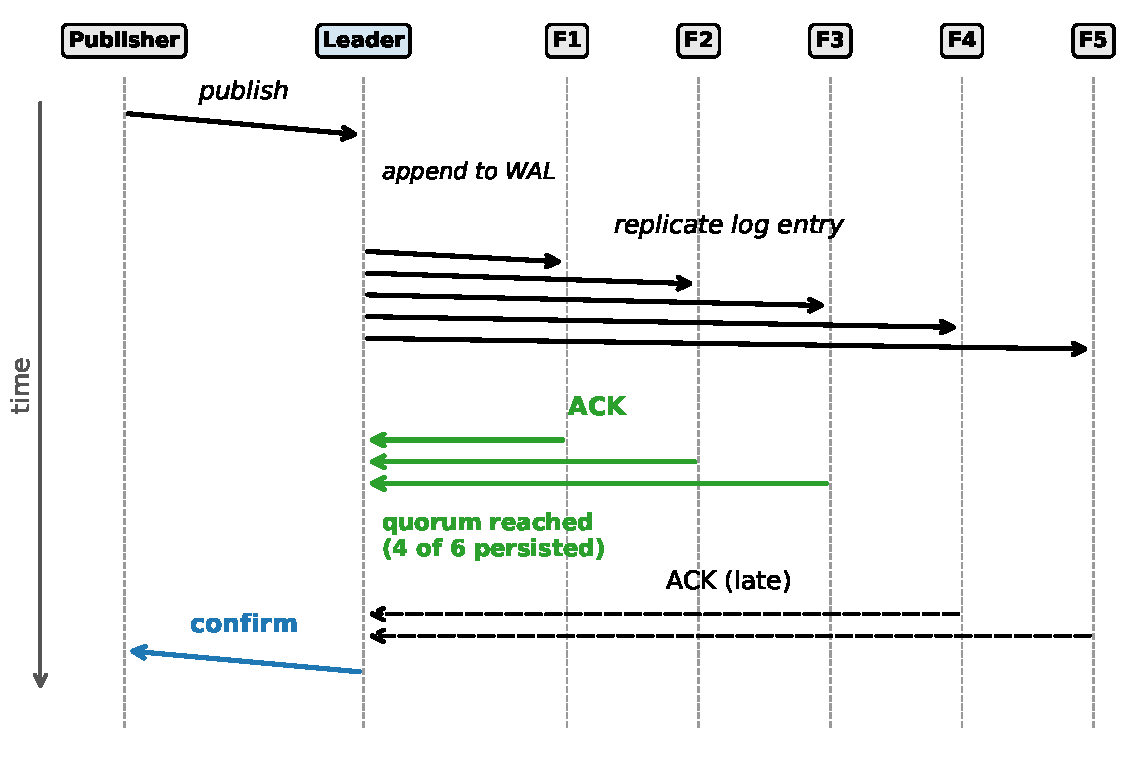
\includegraphics[width=1.04\columnwidth]{../results/plots/0A_raft_replication.pdf}
\caption{Raft replication sequence for a 6-node quorum queue. The leader appends the message to its WAL, replicates to all followers and confirms to the publisher once a quorum (4 of 6) has persisted the entry.}
\label{fig:raft_replication}
\end{figure}

\subsection{Publisher Confirms}
By default, AMQP publishers receive no feedback on whether a message was successfully enqueued. RabbitMQ's publisher confirms extension addresses this by having the broker acknowledge each message after it has been committed~\cite{rmq_confirms_docs}. For quorum queues, this means the confirm is only sent after the Raft commit, making confirms a signal that the message has been replicated to a majority of nodes.

Publisher confirms can operate in two modes. In \textit{synchronous} mode, the publisher waits for each confirm before sending the next message. This serializes publishes and measures the round-trip latency of the Raft replication. In \textit{asynchronous} mode, the publisher sends messages continuously and processes confirms as they arrive, allowing multiple messages to be in flight simultaneously. This pipelined approach achieves higher throughput at the cost of more complex flow control. Both modes are used in our benchmark experiments to benchmark cluster performance under different scenarios.
